\documentclass[a4paper,11pt]{report}

\usepackage{amsmath}
\usepackage{graphicx}
\usepackage{empheq,etoolbox}
% Update display of subequation numbering (Xy) > (X.y)
\patchcmd{\subequations}% <cmd>
  {\theparentequation\alph{equation}}% <search>
  {\theparentequation.\alph{equation}}% <replace>
  {}{}% <success><failure>

\begin{document}

\section*{Single phase flow: governing equation}

We write incompressible Navier-Stokes equations as

\begin{subequations}
    \label{eqn:NavierStokes}
    \begin{empheq}[left=\empheqlbrace]{align}
        &\nabla \cdot \vec{u} = 0 \label{eqn:continuity}\\
        &\rho\left(\partial_t \vec{u} + \vec{u} \cdot \nabla \vec{u}\right) = -\nabla p + \mu \nabla^2 \vec{u} + \rho \vec{f} \label{eqn:momentum}
    \end{empheq}
\end{subequations}
%
with $\vec{u} = \vec{u}\left(\vec{x},t\right)$ the velocity field, $p = p(\vec{x},t)$ the pressure field, $\rho$ the density,
$\mu$ the viscosity and $\vec{f} = \vec{f}\left(\vec{x},t\right)$ external volume forces.

\section*{Time discretization: predictor-corrector}

The unknowns in \eqref{eqn:NavierStokes} are $\vec{u}$ and $p$. A 2nd-order central scheme time discretization of equation \eqref{eqn:momentum}, which contains both variables at new timestep, correspond to
\begin{equation}
    \label{eqn:2ndOrderTime}
    \begin{aligned}
        &\frac{\vec{u}^{\, n+1} - \vec{u}^{\, n}}{\Delta t} = \\
        &= \frac{1}{\rho}\left[-\nabla p^{n+1} - \vec{u}^{\, n+1/2} \cdot \nabla \vec{u}^{\, n+1/2} + \mu \nabla^2 \vec{u}^{\, n+1/2} + \rho \vec{f}^{\, n+1/2}\right]
    \end{aligned}
\end{equation}
with $\vec{u}^{\, n} = \vec{u}\left(\vec{x},n\Delta t\right)$.
We replace the pressure $p^{n+1}$ with the value at actual timestep $p^n$, so the updated velocity field does not satisfy mass conservation
\begin{equation}
    \label{eqn:predict}
    \frac{\vec{u}^{\, *} - \vec{u}^{\, n}}{\Delta t} = -\frac{1}{\rho}\nabla p^n + \frac{3}{2}\vec{\mathcal{H}}^{\, n} - \frac{1}{2}\vec{\mathcal{H}}^{\, n-1} + \vec{f}^{\, n+1/2}\\
\end{equation}
where $\mathcal{H}_i = -u_j\partial_j u_i + \nu \partial_j \partial_j u_i$ and we have extrapolated values at timestep $n+1/2$ using values from timestep $n$ and $n-1$ (2nd order Adams-Bashfort scheme). We call this predicted velocity field $u^{*}$. To enforce mass conservation we introduce a function $\phi = \phi\left(\vec{x},t\right)$ such that
\begin{equation}
    \label{eqn:correct}
    \vec{u}^{\, n+1} = \vec{u}^{\, *} - \frac{\Delta t}{\rho}\nabla \phi^{\, n}
\end{equation}
and $\phi$ must satisfy the condition
\begin{equation}
    \label{eqn:Poisson}
    \nabla^2 \phi^{\, n} = \frac{\rho}{\Delta t}\nabla \cdot \vec{u}^{\, *}
\end{equation}
The sum of equations \eqref{eqn:predict} and \eqref{eqn:correct} shows that (by comparison with \eqref{eqn:2ndOrderTime})
\begin{equation}
    p^{n+1} = p^{n} + \phi^{n}
\end{equation}
hence, $\phi^n$ represent the pressure increment at timestep $n$ which satisify mass conservation.

\section*{Space discretization}

We use a staggered grid, as shown in figure \ref{fig:grid}. We replace space coordinates as $\vec{x} = (x,y) = ((i + s_x)\Delta x,(j + s_y)\Delta y)$, where $i = 1,2,\dots,N_x$, $j = 1,2,\dots,N_y$ are integers, $\Delta x$ and $\Delta y$ are the grid spacing in $x$ and $y$ direction (\emph{i.e.} $\Delta x = L_x/N_x$ and $\Delta y = L_y/N_y$); $s_x$ and $s_y$ are coefficient to get the value at cell center of cell face. Pressure is defined at cell center ($s_x = -0.5$, $s_y = -0.5$), while velocity on cell faces: for horizontal velocity component $s_x = 0$, $s_y = -0.5$, while for vertical velocity component $s_x = -0.5$, $s_y = 0$.

\begin{figure}[ht]
    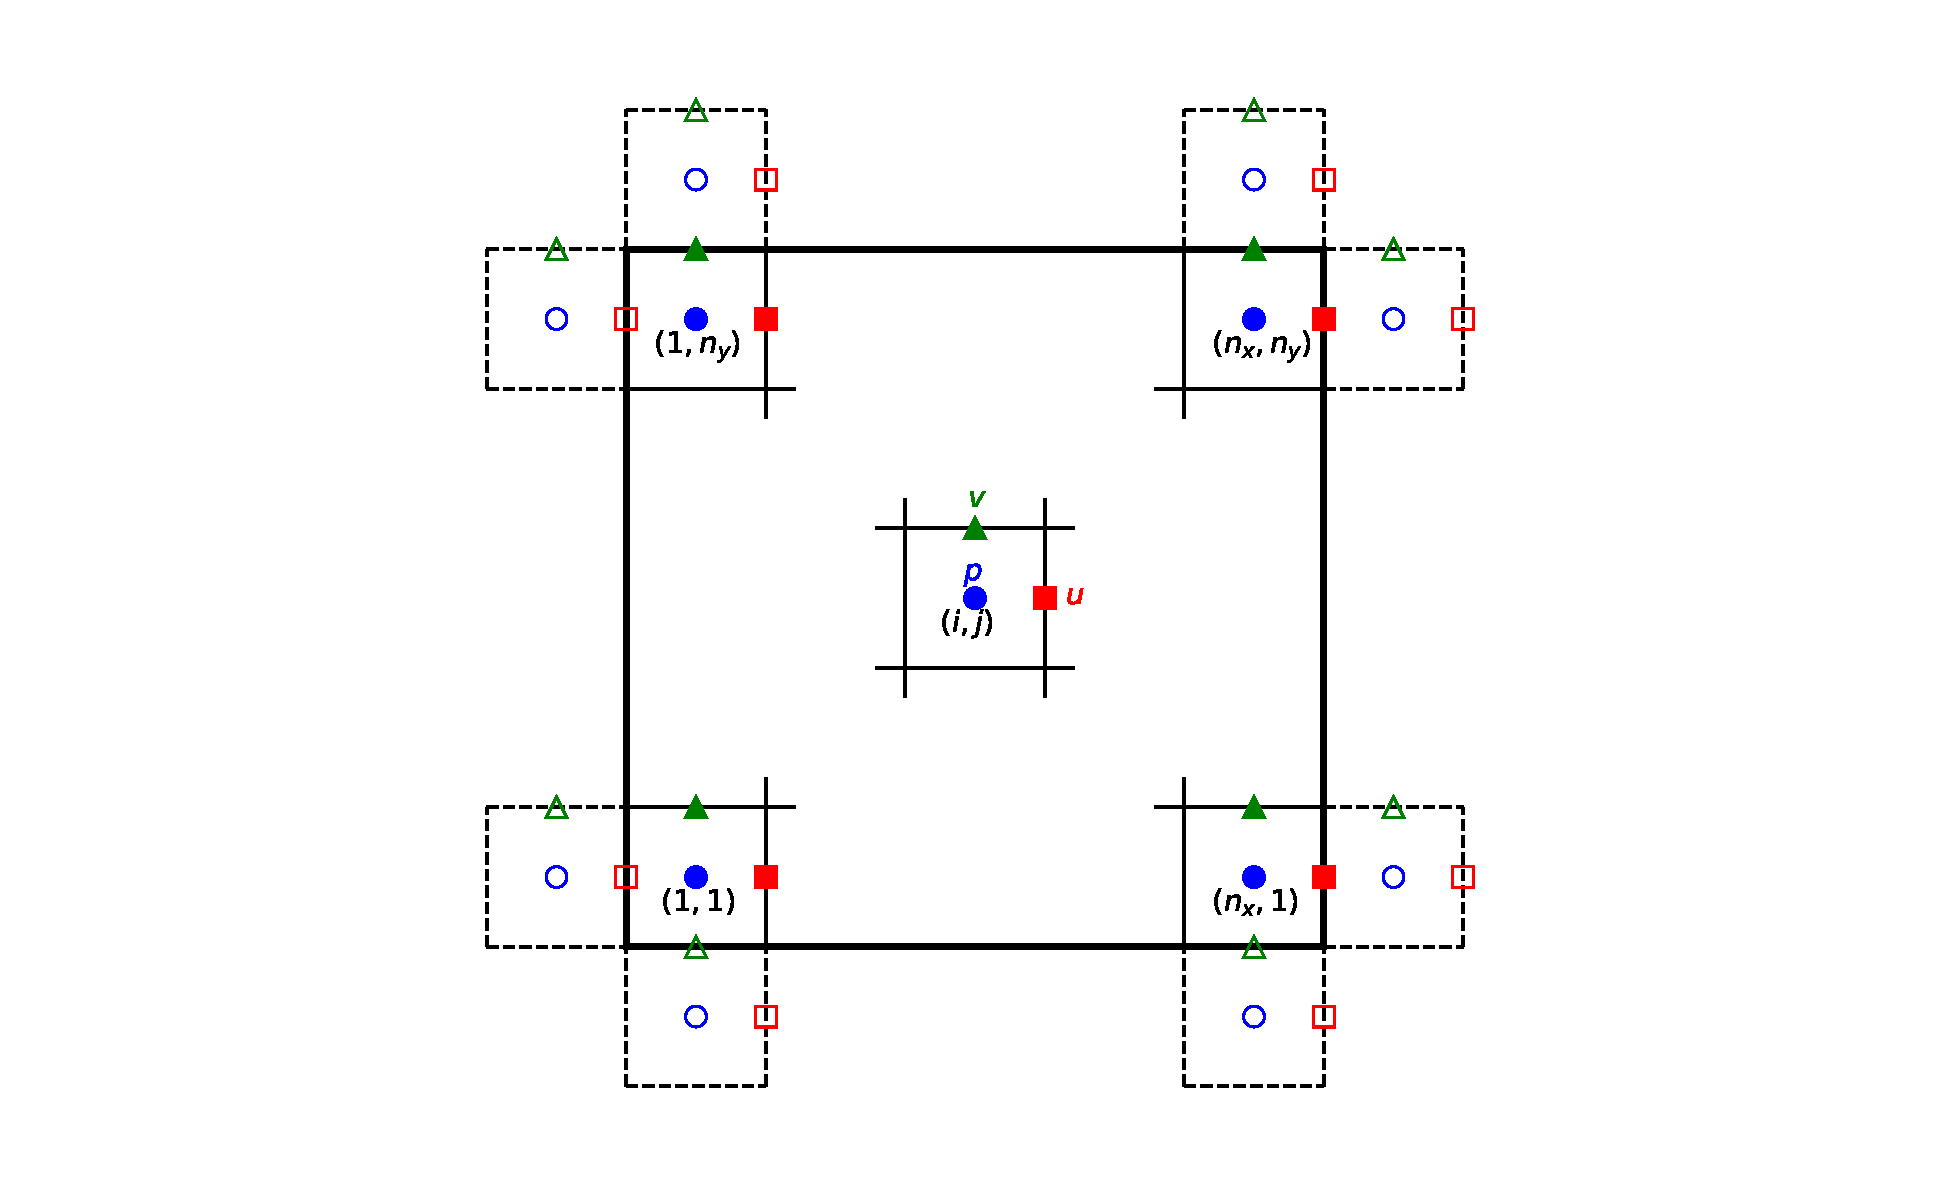
\includegraphics[width=\textwidth]{grid.eps}
    \caption{Sketch of the computational grid. Empty symbols represent ghost nodes.\label{fig:grid}}
\end{figure}

By using the staggered grid the pressure gradient term in the $x$ component of equation \eqref{eqn:momentum}, for example, can be expressed as
\begin{equation*}
    \partial_t u + \dots \approx -\frac{1}{\rho}\frac{p_{i+1,j} - p_{i,j}}{\Delta x} + \dots
\end{equation*}
and correspond to a 2nd order central scheme approximation of the pressure gradient on the $x$-face of cell $(i,j)$ (red square in figure \ref{fig:grid}). The diffusion term, in the same equation can be approximated with 2nd order accuracy as
\begin{equation*}
    \left . \nabla^2 u \right |_{i,j} \approx \nu \frac{u_{i+1,j} - 2u_{i,j} + u_{i-1,j}}{\Delta x^2}.
\end{equation*}
For incompressible flows we can write
\begin{equation*}
    \begin{aligned}
        \frac{\partial uu}{\partial x} + \frac{\partial uv}{\partial y} = u\frac{\partial u}{\partial x} + &u\frac{\partial u}{\partial x} + u\frac{\partial v}{\partial y} + v\frac{\partial u}{\partial y} = \\ 
        & = u\frac{\partial u}{\partial x} + v\frac{\partial u}{\partial y} + u\underbrace{\left(\frac{\partial u}{\partial x} + 
        \frac{\partial v}{\partial y}\right)}_{\nabla \cdot \vec{u} = 0} = u\frac{\partial u}{\partial x} + v\frac{\partial u}{\partial y}
    \end{aligned}
\end{equation*}
A 2nd order approximation of the advection term in $x$ direction can be written as
\begin{equation*}
    \begin{aligned}
        \left . \frac{\partial uu}{\partial x}\right |_{i,j} \approx& \frac{\left(uu\right)_{i+1/2,j} - \left(uu\right)_{i-1/2,j}}{\Delta x} = \\
        & = \left[\frac{\left(u_{i+1,j} + u_{i,j}\right)^2}{4} - \frac{\left(u_{i,j} + u_{i-1,j}\right)^2}{4}\right]\frac{1}{\Delta x}
    \end{aligned}
\end{equation*}
\begin{equation*}
    \begin{aligned}        
        \left . \frac{\partial uv}{\partial y}\right |_{i,j} &\approx \frac{uv_{i,j+1/2} - uv_{i,j-1/2}}{\Delta y} = \\
        &\left[\frac{u_{i,j+1} + u_{i,j}}{2}\frac{v_{i+1,j} + v_{i,j}}{2} - \frac{u_{i,j} + u_{i,j-1}}{2}\frac{v_{i+1,j-1} + v_{i,j-1}}{2} \right]\frac{1}{\Delta y}
    \end{aligned}
\end{equation*}

\section*{Poisson Solver}

\end{document}